\chapter{Entwicklung der BMS-Algorithmus}\thispagestyle{fancy}


\section{Einf�hrung in die Batterie Management System}
\large{Die Batterie-Management-System ist ein System, welches in Abteilung Embedded Systeme entstanden ist, der zu �berwachung von Batteriezellen entwickelt wurde. Die BMS messen Spannung, Temperatur und Leitwert an jeweiligen Zellen. Eine BMS-Platine kann man mit 12 Zellen verbinden und von allen den Spannungswert auslesen. Der BMS wurde in der Batteriespeicher in Alt Daber im Brandenburg zur Betrieb genommen. Es soll vor allem als �berwachungssystem f�r die Firma dienen, damit man die Spannungen und andere Werten kontrollieren kann. Dazu wird, f�r bessere �bersichtlichkeit und Orientierung, eine Visualisation angefertigt. (siehe Abbildung(hier einen Bild Visualisation). Die Daten von jeweiligen Batteriezellen sind in falschen Reihenordnung gespeichert. Dies ist wegen die gef�hrte Leitung von Kommunikationskabeln verursacht. Dabei ist meine Aufgabe ein Algorithmus entwickeln, der die Daten in die richtige, von uns festgestellte, Reihenordnung sortiert. Damit sollen die Messwerten richtig in der Visualisation gezeigt werden. }


\section{Erstellung eines BMS-Planes}
\large{Die Batterien sollen mit dem BMS-System belegt werden. Daf�r war ein Plan zur Verteilung von BMS Platinen konzipiert. Es waren mehrere Versionen entstanden, wie die Platinen verbunden werden. Wichtige Punkten waren, dass die Kommunikationskabeln nicht l�nger als das festgelegte Maximum werden und dass die Batteriezellen mit dem BMS System verbunden werden. Der Plan sollte �bersichtlich sein, weil es f�r die Orientierung in dem EBU dienen soll. Der Plan wurde mit dem Microsoft Word erstellt. Nach eine Gruppenbesprechung wurde die Nummerierung der jeweilige Teilen der EBU. In einen EBU gibt es 16 Trog-Verbunde mit jeweils 5 Tr�gen. Ein Trog hat zwei Zellenbl�cke mit jeweils 6 Zellen. Eine Platine kann Werten von zwei Zellenbl�cken messen. Die Platine reicht aber mit Kabeln nicht �ber einen Trog, das hei�t, dass die BMS-Platine die Werten von zwei nebenstehenden Zellenbl�cke messen kann.\\
In der erste Plan (siehe Abbildung \ref{Plan_Trogverbund} und \ref{plan_legende}).) ist die Verteilung und Nummerierung zu sehen.\\

\begin{figure}[htbp]
  \centering
     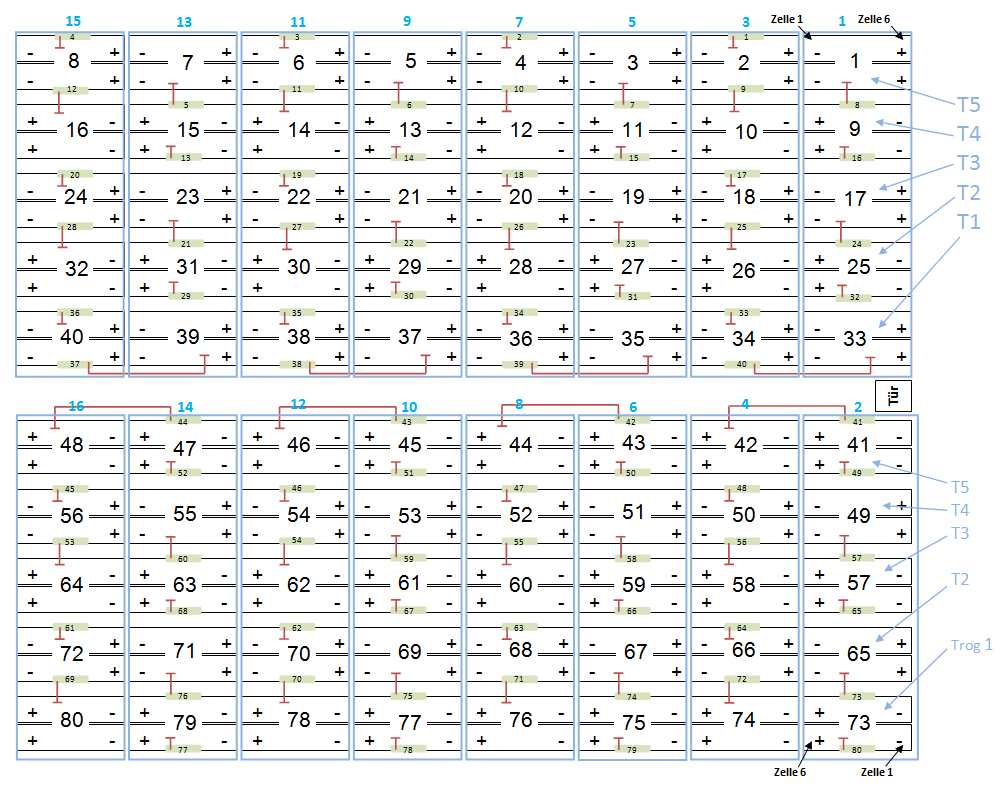
\includegraphics[width=0.99\textwidth]{images/Plan_Trogverbund.png}
  \caption{Plan mit Beschriftung}
  \label{Plan_Trogverbund}
\end{figure}

\begin{figure}[htbp]
  \centering
     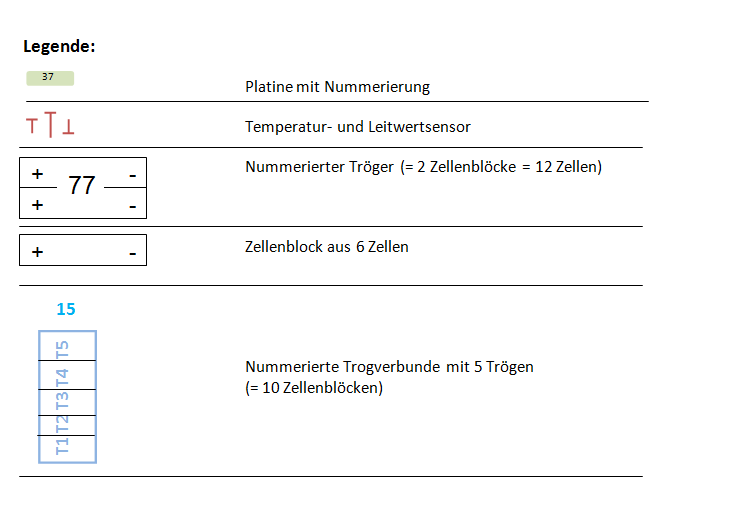
\includegraphics[width=0.8\textwidth]{images/plan_legende.png}
  \caption{Die Legende zum Plan}
  \label{plan_legende}
\end{figure}

In den zweiten Plan geht es haupts�chlich um das Verkabelung zwischen BMS-Platinen. Die Platinen wurden mit Kommunikationskabeln verbunden. Dies ist mit blau gezeichnet (siehe Abbildung \ref{Montage_plan}).

\begin{figure}[htbp]
  \centering
     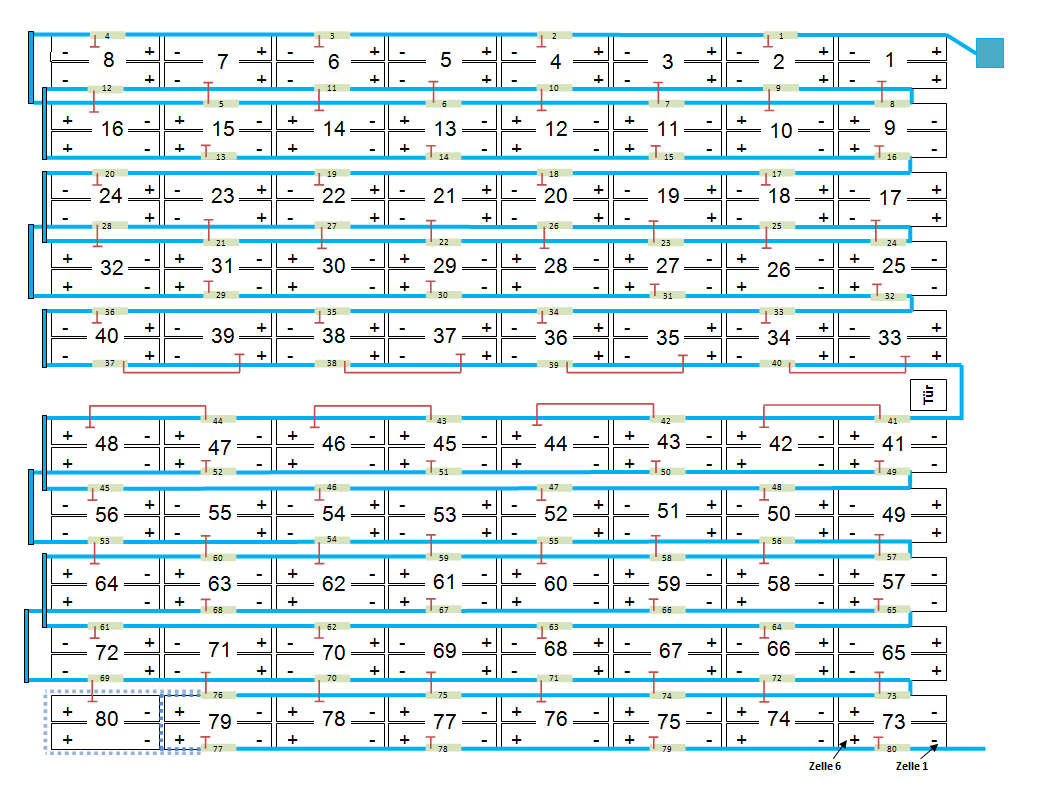
\includegraphics[width=1\textwidth]{images/Montage_plan.png}
  \caption{Verkabelung von Platinen}
  \label{Montage_plan}
\end{figure}
\pagebreak


\section{Entwicklung der Algorithmus}
\large{Zu n�chst wurden Tabellen im Excel erstellt. Die erste Tabelle beinhaltet Informationen zur Verteilung von Platinen. Aus dieser Tabelle sollte man schnell die Nummer der Platine auslesen, welche zum Beispiel die Batteriezelle Nummer 5 des Troges 2 des Trog-Verbundes 11 messen wurde (siehe Tabellen \ref{tbl:tabelle_excel}). Diese Tabelle dient f�r die bessere Orientierung in einen EBU. \\ 
In der n�chste Tabelle ist der Zusammenhang zwischen eingeladene und festgestellte Werte-Indexen beschrieben. Aus diese Tabelle sollte man zum Beispiel auslesen, dass die Platine Nummer 1 die Indexen 0 bis 14 mit Werten von 5. Trog des 1. und 3. Trog-Verbundes beladet. Die Indexen 0 bis 14 werden mit Werten beladen, aber damit es sortiert wird, muss man die Indexen auf die festgesetzte Indexen aufladen, in diesem Fall wurden es Indexen von 210 bis 215, von 60 bis 65 und drei Indexen 222, 223 und 224 (siehe Tabelle \ref{tbl:example_tabelle_indexing}). Die Visualisierung wird die festgelegte Anordnung anzeigen. \\


\begin{table}
  \caption{Tabelle mit Trogverbund und Reihenordnung}
  \label{tbl:tabelle_excel}
	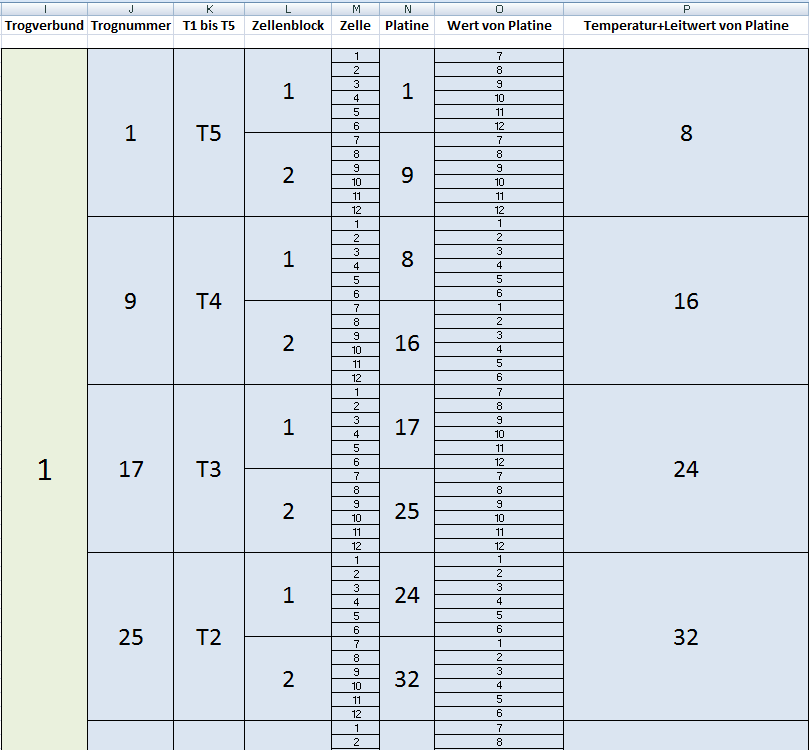
\includegraphics[width=\linewidth]{images/example2_tabelle_excel.png}
\end{table}

% Die Excel Tabellen erstellt, einen System gefunden, sehr viel Berechnen, logische Denken, Spannungswerten, Temperatur, Leitwert, Error

\begin{table}
  \caption{Tabelle mit Indexen}
  \label{tbl:example_tabelle_indexing}
  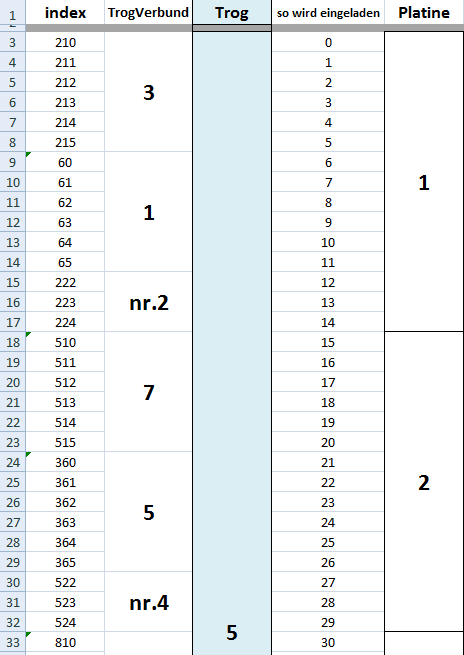
\includegraphics[width=\linewidth]{images/example_tabelle_indexing.png}
\end{table}

Nach dem die Fakten gesammelt wurden, kann man den Algorithmus entwickeln. Man muss die Zusammenh�nge finden und davon allgemeine Regeln bilden. Diese Regeln m�ssen alle Werte-Indexen beschreiben. Dann sind die Regeln zusammengefasst und wie m�glich wird es vereinfacht. Diese Vereinfachungen wurden erstens mit Programmiersprache C beschreiben. Mit If- und Switch-Operatoren und for-Schleifen wurde die Zuordnung der jeweiligen Werte-Index auf die von uns festgestellte Indexen durchgef�hrt.\\ %siehe Anhang mit dem Algorithmus

Die Visualisierung von der BMS Daten erfolgt �ber die B\&R Umgebung, welche die Sprache \textbf{ST} benutzt. Der Code in C war in die Sprache ST umgewandelt und dann in die Umgebung eingesetzt. }%siehe Screenshot von Johann

\pagebreak

\section{Test Durchf�hrung}
\large{Nach der Anwendung in die Visualisation wurde der Algorithmus getestet. Der Test war folgendes durchgef�hrt: man muss das, was die Visualisation zeigt, mit Werten eines Messger�tes an eine Zelle vergleichen. Es wurde an allen Zellen getestet ob die Werten �bereinstimmen. Der Test hat positiven Ergebnis, das hei�t, dass die Werten auf richtigen Indexen gespeichert sind.}

\section{Fazit}
\large{Mit der richtigen Zuordnung der Messwerte kann man den Mitarbeitern oder Kunden zeigen, welche Spannung an den jeweiligen Batteriezellen anliegt. Auch die Temperaturen und Leitwerten sind damit unter Aufsicht. Die ganze Funktionalit�t wird mittels Visualisation �berwacht. (Screenshots von Johann)}